If we assume that a stellar population forms
impulsively in the distant pass with IMF $\mu(m_*)$(with minimum mass
$m_0$ and maximum mass $m_1$), then the surviving mass fraction at any
future time $t$ is given by
\begin{equation}
f(t) =\frac{ \int_{m_0}^{m_{\rm T}(t)} m_* \mu(m_*) dm_* }{ \int_{m_0}^{m_1} m_* \mu(m_*) dm_* },
\end{equation}
where the main sequence turnoff mass is approximately
\begin{equation}
m_{\rm T}(t) \approx 2.5M_\odot~ \left( \frac{t}{10^9~{\rm yr}} \right)^{-0.4}.
\end{equation}
For a Salpeter IMF $\mu(m_*) \propto m_*^{-2.35}$ with $m_0=0.1M_\odot$ and $m_1=100M_\odot$,
\begin{equation}
f_{\rm Sal}(t) = 1.098 - 0.490 \left(\frac{t}{10^{10}~{\rm yr}} \right)^{0.14}
\end{equation}
{\bf NCS: we should probably use a Kroupa/Chabrier IMF, but this gets the ball rolling.}
If we approximate post-main sequence evolution as instantaneous and define $\lambda(m_*)$ as the fractional mass lost during all stages of stellar evolution, then the mass loss rate density
\begin{equation}
q(t) = \frac{\rho_*}{\bar{m}_*} \lambda(m_{\rm T}(t)) m_{\rm T}(t) \frac{df}{dt},
\end{equation}
where the mean stellar mass $\bar{m}_* = \int_{m_0}^{m_{\rm T}(t)} m_*\mu(m_*)dm_* \approx 0.3 M_\odot$.  Further approximating $\lambda(m_*)=0.5$, and using the Salpeter IMF once more, gives
\begin{equation}
q(t) = \frac{\rho_*}{10^{10}~{\rm yr}} \times 0.11 \left(\frac{t}{10^{10}~{\rm yr}} \right)^{-1.26}.
\end{equation}
This is a specific, time-dependent definition of $\eta(t) (=0.11(t/t_{\rm h})^{-1.26})$; if we consider different star formation scenarios (for example, continuous star formation) or different IMFs, it will change.  Once these free parameters are specified, however, we can answer an important question: do young stellar populations increase or decrease the SMBH feeding rate $\dot{M}$?  Clearly, $\eta(t)$ is larger for young stellar populations, but these stars also have high wind velocities that diminish the stagnation radius.  Crudely approximating $v_{\rm w}=75~{\rm km~s}^{-1}$ for $m_{\rm T} < 10M_{\odot}$ and $v_{\rm w}=3000~{\rm km~s}^{-1}$ for $m_{\rm T} > 10M_{\odot}$ (motivated by the transition from dust-driven wind loss on the AGB to line-driven wind loss from Wolf-Rayet stars), we can employ the relation $\dot{M} \propto \eta(t) r_{\rm s}^{2-\Gamma}\propto \eta(t) v_{\rm w}^{-4+2\Gamma}$ (where $\rho_* \propto r^{-\Gamma}$) to determine the impact of stellar ``youth'' on SMBH feeding rates.
{\bf AG:As I previously mentioned this discussion of the eta is not
  quite correct...}
\begin{figure}
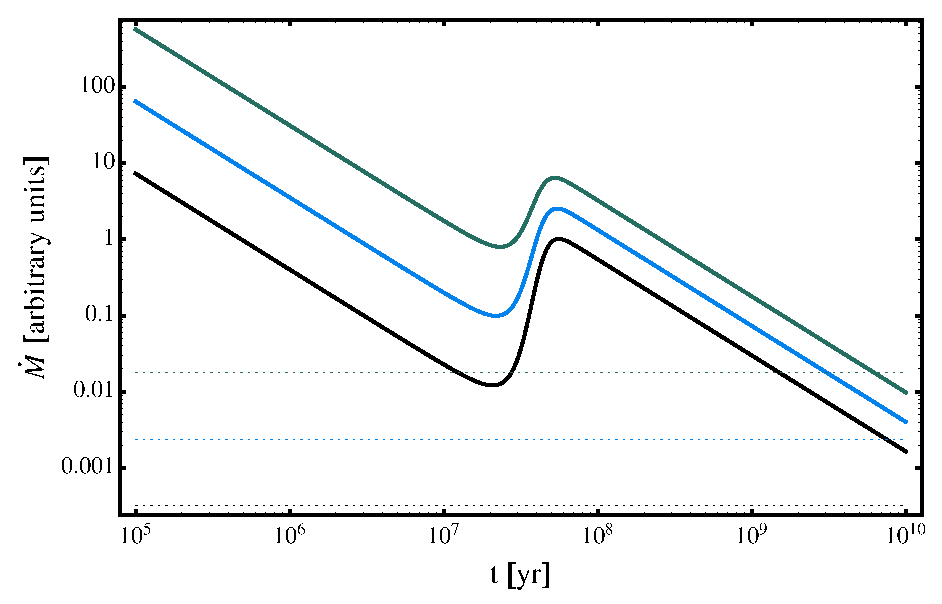
\includegraphics[width=\columnwidth]{NickPlot.eps}
\caption{\label{NickPlot} SMBH feeding rates $\dot{M}=\eta(t) \times M_*(r_{\rm s})$, in arbitrary units.  The green, blue, and black curves are for galaxies with $\Gamma$ values of $0.1$, $0.5$, and $0.9$, respectively.  Solid curves represent impulsive-mode star formation, while dotted curves represent continuous-mode star formation. {\bf NCS: I think these old continuous curves are wrong, need to revise}}
\end{figure}

In Fig. \ref{NickPlot} we plot $\dot{M}$, in arbitrary units, as a
function of time, for three different stellar density profiles $\Gamma
= \{1.1, 1.5, 1.9\}$ (which are normalized to have the same mass at an
influence radius $r _{\rm soi}=10~{\rm pc}$ around a $10^7M_\odot$
SMBH).  We parametrize the wind velocity as
\begin{equation} \frac{v_{\rm w}}{3000 ~\rm
km~s^{-1}}=520-495\tanh\left( \frac{t-10^{7.5}~{\rm yr}}{10^{7}~{\rm
yr}}\right). \label{NickV1}
\end{equation} This counts Type II SNe heating as ``winds;'' if
instead we are in the portion of parameter space where $r_{\rm II}$ is
very large, then we use the alternate parametrization
\begin{equation} \frac{v_{\rm w}}{3000 ~\rm
km~s^{-1}}=520-495\tanh\left( \frac{t-10^{7}~{\rm yr}}{10^{6.5}~{\rm
yr}}\right), \label{NickV2}
\end{equation} which only allows short lived Wolf-Rayet stars to
contribute to the high-heating mode.  The ``impulsive burst'' mode of
star formation produces large ($\sim 10$) differences between the
three $\dot{M}$ curves at early times, when $r_{\rm s}$ is small, but
smaller ($\sim 3$) differences at late times, when $r_{\rm s}$ is
large.  We also plot, as dotted curves, a simple model for the
``continuous'' mode of star formation, where mass loss is calculated
as $\bar{\eta} = \int\eta(t)dt/t_{\rm h} \approx 4$ and an average
energy injection in the wind is calculated as $\bar{v_{\rm
w}^2}=\int\eta(t)v_{\rm w}^2(t)dt/\bar{\eta} \approx (800~{\rm
km~s}^{-1})^2$.  Interestingly, the continuous mode of star formation
produces small differences from late-time $\dot{M}$ seen in cusp
galaxies with impulsive star formation; however, continuous mode star
formation decreases late-time $\dot{M}$ by an order of magnitude
relative to impulsive star formation in core galaxies.  {\bf NCS: I
think this old discussion of MDot in the continuous limit is wrong,
need to revise}

The continuous mode of star formation can be studied more accurately
by including arbitrary star formation histories $S(t)$, measured in
units of mass per time.  In particular, if an impulsively formed
stellar population that is $t$ years of age, we can write its current
mass loss rate, $\dot{\bar{m}}(t)$, and its current effective wind
speed, $\bar{v}_{\rm w}(t)$.  Specifically,
\begin{align} 
  \dot{\bar{m}}(t) &= \frac{\Delta M(t) \mu(M_{\rm TO}(t))
    \left|\dot{M}_{\rm TO}(t)\right| + f_{\rm ms} \int_{m_0}^{m_{\rm
        T}(t)}
    \dot{m}(m_*, t) \mu(m_*) {\rm d}m_* }{\bar{m}_*}\\
  \dot{\bar{e}}(t) &=\dot{e}_{\rm TO}+ f_{\rm MS} \int_{m_0}^{m_{\rm T}(t)}
  \frac{\vw^2(t) \dot{m}(m_*, t) \mu(m_*) {\rm d}m_*}{\bar{m}_*}.
\end{align} 

The first term corresponds to a more impulsive contribution from
post-main sequence (PMS) stars, while the second term corresponds to
the contribution from main-sequence winds. 


{\bf Note that I have not written the turnoff contribution in terms of
  a wind velocity. One can simply read off the specific energy
  injection rate from Voss '09...}

The effective wind velocity in the impulsive limit may then be written
as 

\begin{align}
\bar{v}_w=2 \dot{\bar{e}}/\dot{\bar{m}}
\end{align}

We can then use these integrated quantities to determine the effective
$V_w$ for arbitrary star formation histories.

\begin{align} 
  \dot{M}(t) &= \int_0^t S(t_1) \dot{\bar{m}}(t-t_1){\rm
      d}t_1\\
  \dot{E}(t) &= \int_0^t S(t_1) \dot{\bar{e}}(t-t_1){\rm
      d}t_1\\
  V_w^2(t) &=2 \dot{E}(t)/\dot{M}(t)
\end{align}

\begin{figure}
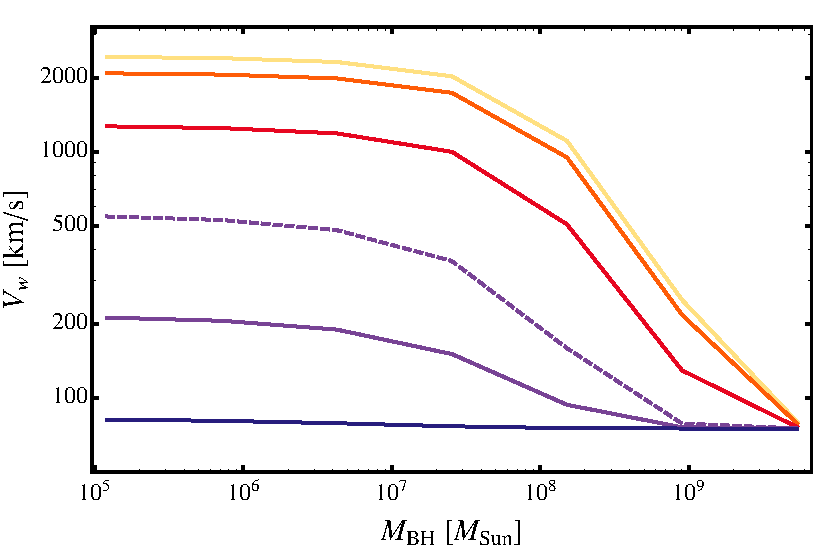
\includegraphics[width=\columnwidth]{vw.pdf}
\caption{\label{NickPlot2} Effective wind velocities $V_{\rm w}$ for
different $S(t)$.  The yellow and orange curves are the Moster SF
histories, with and without Type II SNe, respectively.  The red,
purple, and blue curves are Moster SFs convolved with a $\sin^2(t)$
function normalized to $10^7$, $10^8$, and $10^9$ yr fluctuations,
respectively.  These solid curves lack SN, but the dashed purple curve
possesses it.  Effective $V_{\rm w}$ is strongly diminished when the
variability timescale is greater than $\sim$ twice the duration of
high-velocity winds.}
\end{figure}

We show $V_{\rm W}$ for different star formation histories in
Fig. \ref{NickPlot2}.  In particular, we use Eqs. 17-20 from Moster et
al and the $M_{\rm BH}-M_{\rm halo}$ relation from Bandara et al {\bf
(NCS: add real refs)} to define $S(t)$ for particular galaxies.  It
seems that ``bumpy'' SF histories severely diminish $V_{\rm w}$ if the
timescale for SF variability is a factor of a few or more greater than
the duration of high-velocity winds (either 10 or 40 Myr).

%%% Local Variables: 
%%% mode: latex
%%% TeX-master: "ms"
%%% End: 
